\documentclass[11pt]{article}
%\documentclass[runningheads]{llncs}
\usepackage[margin=1in]{geometry}
\usepackage{fullpage}
\usepackage{amsmath,amsfonts,amsthm}
\usepackage{amsmath,amsfonts}
\usepackage{mathrsfs}
\usepackage{mathpazo}
\usepackage{hyperref}
\renewcommand\UrlFont{\color{blue}\rmfamily}
\usepackage{graphicx}
\usepackage{xspace}
\usepackage{endnotes}
\usepackage{color}
\usepackage{bm}
\usepackage{times}
\usepackage{amssymb,latexsym}
\usepackage{enumitem}
\usepackage{caption}
\usepackage{tikz}
\usepackage{multirow}
\usepackage{floatrow}
\usepackage{float}
\usepackage{ragged2e}
\usepackage{wrapfig}
\usepackage[normalem]{ulem}
\usepackage{subcaption}
\captionsetup{compatibility=false}
\newtheorem{theorem}{Theorem}
\newtheorem{proposition}[theorem]{Proposition}
\newtheorem{conjecture}[theorem]{Conjecture}
\newtheorem{lemma}[theorem]{Lemma}
\newtheorem{claim}[theorem]{Claim}
\newtheorem{fact}[theorem]{Fact}
\newtheorem{corollary}[theorem]{Corollary}

\newtheorem{remark}[theorem]{Remark}

\newtheorem{definition}[theorem]{Definition}
\newtheorem{example}[theorem]{Example}


\newcommand{\meas}{
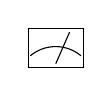
\begin{tikzpicture}
\filldraw[fill=white] (0,.25) rectangle (.7,-.25);
\draw (.67,-.1) arc (50:130:.5);
\draw (.35,-.2)--(.525,.2);
\end{tikzpicture}
}

\newcommand{\beq}{\begin{eqnarray}}
\newcommand{\eeq}{\end{eqnarray}}

\newcommand{\ket}[1]{|#1\rangle}
\newcommand{\bra}[1]{\langle#1|}
\newcommand{\kb}[1]{|#1\rangle\langle#1|}
\newcommand{\proj}[1]{\ket{#1}\!\bra{#1}}
\newcommand{\Tr}{\mbox{\rm Tr}}
\newcommand{\Id}{\ensuremath{\mathop{\rm Id}\nolimits}}
\newcommand{\Es}[1]{\ensuremath{\mathop{\textsc{E}}}_{#1}}

\newcommand{\CON}{C}
\newcommand{\DIS}{d}
\newcommand{\Drho}{\DIS_\rho}
\newcommand{\Trho}{\Tr_\rho}


\newcommand{\setft}[1]{\mathrm{#1}}
\newcommand{\Density}{\setft{D}}
\newcommand{\Pos}{\setft{Pos}}
\newcommand{\Proj}{\setft{Proj}}
\newcommand{\Obs}{\setft{Obs}}
\newcommand{\Channel}{\setft{C}}
\newcommand{\Unitary}{\setft{U}}
\newcommand{\Herm}{\setft{Herm}}
\newcommand{\Lin}{\setft{L}}
\newcommand{\Trans}{\setft{T}}
\DeclareMathOperator{\poly}{poly}

\newcommand{\reg}[1]{{\textsf{#1}}}

\newcommand{\norm}[1]{\left\|#1\right\|}

\newcommand{\C}{\ensuremath{\mathbb{C}}}
\newcommand{\N}{\ensuremath{\mathbb{N}}}
\newcommand{\F}{\ensuremath{\mathbb{F}}}
\newcommand{\K}{\ensuremath{\mathbb{K}}}
\newcommand{\R}{\ensuremath{\mathbb{R}}}
\newcommand{\Z}{\ensuremath{\mathbb{Z}}}

\newcommand{\mD}{\mathcal{D}}
\newcommand{\mH}{\mathcal{H}}
\newcommand{\mT}{\mathcal{T}}
\newcommand{\Alg}{\mathcal{A}}
\newcommand{\mM}{\mathcal{M}}
\newcommand{\mC}{\mathcal{C}}
\newcommand{\mR}{\mathcal{R}}

\newcommand{\eps}{\varepsilon}
\newcommand{\ph}{\ensuremath{\varphi}}

\newcommand{\Acc}{\textsc{Acc}}
\newcommand{\Samp}{\textsc{Samp}}
\newcommand{\Ext}{\ensuremath{\text{Ext}}}

\newcommand{\Hmin}{H_\infty}
\newcommand{\Hmax}{H_{\ensuremath{\text{max}}}}

\newcommand{\CHSH}{{\rm CHSH}}
\newcommand{\EPR}{{\rm EPR}}
\newcommand{\MS}{{\rm MS}}
\newcommand{\basis}{\mathcal{B}}
\newcommand{\pauli}{\mathcal{P}}
\newcommand{\paulip}{\tilde{\mathcal{P}}}
\newcommand{\pbt}{\textsc{pbt}}
\newcommand{\qauli}{\mathcal{Q}}
\newcommand{\rauli}{\mathcal{R}}
\newcommand{\raulip}{\tilde{\mathcal{R}}}
\newcommand{\qaulip}{\tilde{\mathcal{Q}}}
\newcommand{\magic}{\mathcal{M}}
\newcommand{\wagon}{\mathcal{W}}
\newcommand{\aux}{\textsc {aux}}
\newcommand{\ctl}{\textsc {ctl}}
\newcommand{\swap}{\textsc {swap}}
\newcommand{\conj}{\textsc{conj}}
\newcommand{\perm}{\textsc{tens}}
\newcommand{\prodt}{\textsc{prod}}
\newcommand{\comt}{\textsc{com}}
\newcommand{\act}{\textsc{ac}}
\newcommand{\idt}{\textsc{id}}
\newcommand{\bellt}{\textsc{Bell}}
\newcommand{\pbellt}{\textsc{ParBell}}

\newcommand{\rigid}{\textsc{rigid}}
\newcommand{\conjc}{\textsc{conj-cliff}}
\newcommand{\ecliff}{\textsc{e-cliff}}
\newcommand{\cliff}{\textsc{cliff}}
\newcommand{\tom}{\textsc{tom}}
\newcommand{\SWAP}{\textsc{SW}}
\newcommand{\clifford}{\mathcal{C}}
\newcommand{\cliffordga}{{\mathcal{C}_1}}
\newcommand{\cliffordgb}{{\mathcal{C}_2}}
\newcommand{\heisg}{{\mathcal{H}^{(1)}}}
\newcommand{\heisgn}{{\mathcal{H}^{(n)}}}
\newcommand{\heisga}{{\mathcal{H}_1}}
\newcommand{\heisgb}{{\mathcal{H}_{2}}}
\newcommand{\cliffordgan}{{\mathcal{C}^{(n)}_1}}
\newcommand{\cliffordgbn}{{\mathcal{C}^{(n)}_2}}
\newcommand{\cliffordn}{G_\mathcal{C}^{(n)}}
\newcommand{\paulig}{G_{\mathcal{P}}}
\newcommand{\pauligb}{G_{\mathcal{P}_2}}
\newcommand{\paulign}{G_{\mathcal{P}}^{(n)}}
\newcommand{\conjn}{\mathcal{J}^{(n)}\!}
\newcommand{\conjr}{\mathcal{J}\!}
\newcommand{\tr}{\mathcal{T}\!}
\newcommand{\epaulin}{\hat{\mathcal{P}}^{(n)}\!}
\newcommand{\tpaulin}{\tilde{\mathcal{P}}^{(n)}\!}
\newcommand{\paulin}{\mathcal{P}^{(m)}\!}
\newcommand{\ver}{\textsc{V}}
\newcommand{\pv}{\textsc{PV}}
\newcommand{\pp}{\textsc{PP}}
\newcommand{\sk}{\ensuremath{\text{sk}}}

\newcommand{\phase}{\Lambda}

\newcommand{\ekeyspace}{\mR_{ek}}
\newcommand{\messagespace}{\mM}
\newcommand{\cipherspace}{\mC}
\newcommand{\mE}{\mathcal{E}}
\newcommand{\HEEnc}{\mbox{HE.Enc}_{pk}}
\newcommand{\QHEKeyGen}{\mbox{QHE.KeyGen}}
\newcommand{\QHEEnc}{\mbox{QHE.Enc}_{pk}}
\newcommand{\QHEEval}{\mbox{QHE.Eval}}
\newcommand{\QHEDec}{\mbox{QHE.Dec}_{sk}}


%\newcommand{\anote}[1]{\textcolor{blue}{\small {\textbf{(Andrea:} #1 \textbf{) }}}}
%\newcommand{\snote}[1]{\textcolor{green}{\small {\textbf{(Stacey:} #1 \textbf{) }}}}
%\newcommand{\agnote}[1]{\textcolor{cyan}{\small {\textbf{(Alex:} #1 \textbf{) }}}}
%\newcommand{\tnote}[1]{\textcolor{red}{\small {\textbf{(Thomas:} #1 \textbf{) }}}}
%\newcommand{\agnew}[1]{\textcolor{cyan}{#1}}
%\newcommand{\agftnote}[1]{\footnote{\textcolor{cyan}{\small {\textbf{(Alex:} #1\textbf{) }}}}}
%\newcommand{\anew}[1]{\textcolor{blue}{#1}}



%\newcommand{\aftnote}[1]{\footnote{\textcolor{blue}{\small {\textbf{(Andrea:} #1 \textbf{) }}}}}

\newcommand{\highlight}[1]{\uline{#1}}


\bibliographystyle{alpha}

\newif\ifnotes\notestrue
%\newif\ifnotes\notesfalse

%\input{../marginnotes}
%\input{marginnotes}

\begin{document}

\title{Verifier-on-a-Leash: new schemes for verifiable delegated quantum computation, with quasilinear resources}
%\titlerunning{VoL: new schemes for verifiable delegated quantum computation}

\author{Andrea Coladangelo\thanks{Department of Computing and Mathematical Sciences, Caltech, Pasadena, USA. acoladan@cms.caltech.edu}
  \and Alex B. Grilo\thanks{QuSoft and CWI, Amsterdam, the Netherlands. alexg@cwi.nl}
  \and Stacey Jeffery\thanks{QuSoft and CWI, Amsterdam, the Netherlands. jeffery@cwi.nl} % Supported by an NWO Veni Innovational Research Grant under project number 639.021.752 and an NWO WISE Grant.}%\inst{2}
  \and Thomas Vidick\thanks{Department of Computing and Mathematical Sciences, Caltech, Pasadena, USA. vidick@cms.caltech.edu}}%\inst{1}}
%%Supported by ERC QCC.
%%Supported by AFOSR YIP award number FA9550-16-1-0495.
%%Supported by an NWO WISE Grant.
%%Supported by NSF CAREER Grant CCF-1553477, AFOSR YIP award number FA9550-16-1-0495, and the IQIM, an NSF Physics Frontiers Center (NSF Grant PHY-1125565) with support of the Gordon and Betty Moore Foundation (GBMF-12500028).
%%
%\authorrunning{A. Coladangelo, A. Grilo, S. Jeffery and T. Vidick}
%% First names are abbreviated in the running head.
%% If there are more than two authors, 'et al.' is used.
%%
%\institute{$^1$
%Department of Computing and Mathematical Sciences, California
%Institute of Technology, Pasadena, USA. 
%CMS, Caltech, Pasadena, USA \\
%\email{ \{acoladan,
%vidick\}@cms.caltech.edu } \\ $^2$ QuSoft and CWI, Amsterdam, the Netherlands \\ \email{\{alexg,
%jeffery\}@cwi.nl}}


\date{}
\maketitle


\begin{abstract}
\input{abstract}
\end{abstract}


\input{body.tex}

\bibliography{delegation}
\appendix




%===========================%
\section{Some simple tests}
\label{sec:clifford-test}
%===========================%

In this appendix we collect simple tests that will be used as building blocks. In Section~\ref{sec:ms} and Section~\ref{sec:elementary} we review elementary tests whose analysis is either immediate or can be found in the literature. In Section~\ref{sec:bell} we formulate a simple test for measurements in the Bell basis and the associated two-qubit SWAP observable. 
Finally, in Section \ref{sec:pauli-group}, we show how to extend the results from \cite{natarajan2016robust} to derive a robust self-test for the $m$-qubit Pauli group. 


\subsection{The Magic Square game}
\label{sec:ms}

We use the Magic Square game~\cite{Mermin90} as a building block, noting that it  provides a robust self-test test for the two-qubit Weyl-Heisenberg group (see Section~\ref{sec:prelim-notation} for the definition). Questions in this game are specified by a triple of labels corresponding to the same row or column from the square pictured in Figure~\ref{fig:ms} (so a typical question could be $(IZ,XI,XZ)$; there are $6$ questions in total, each a triple). An answer is composed of three values in $\{\pm 1\}$, one for each of the labels making up the question. Answers from the prover should be entrywise consistent, and such that the product of the answers associated to any row or column except the last should be $+1$; for the last column it should be $-1$. The labels indicate the ``honest'' strategy for the game, which consists of each prover measuring two half-EPR pairs using the commuting Pauli observables indicated by the labels of his question. 

\begin{figure}[H]
\begin{center}
\begin{tabular}{|c|c|c|}
\hline
$IZ$ & $ZI$ & $ZZ$ \\
\hline
$XI$ & $IX$ & $XX$ \\
\hline
$XZ$ & $ZX$ & $YY$\\
\hline
\end{tabular}
\end{center}
\caption{Questions, and a strategy, for the Magic Square game}
\label{fig:ms}
\end{figure}

The following lemma states some properties of the Magic Square game, interpreted as a self-test (see e.g.~\cite{WBMS16}). 

\begin{lemma}\label{lem:ms-rigid}
Suppose a strategy for the provers, using state $\ket{\psi}$ and observables $W$, succeeds with probability at least $1-\eps$ in the Magic Square game. Then there exist  isometries $V_D:\mH_\reg{D} \to (\C^2\otimes \C^2)_{\reg{D'}}\otimes {\mH}_{\hat{\reg{D}}}$, for $D\in\{A,B\}$ and a state $\ket{\aux}_{\hat{\reg{A}}\hat{\reg{B}}} \in {\mH}_{\hat{\reg{A}}}\otimes {\mH}_{\hat{\reg{B}}}$ such that
$$\big\| (V_A \otimes V_B) \ket{\psi}_{\reg{AB}} - \ket{\EPR}_{\reg{A}'\reg{B}'}^{\otimes 2} \ket{\aux}_{\hat{\reg{A}}\hat{\reg{B}}} \big\|^2 = O(\sqrt{\eps}),$$
and for $W\in \{I,X,Z\}^2 \cup \{YY\}$,
\begin{align*}
\big\| \big(W -V_A^\dagger \sigma_W V_A\big) \otimes \Id_B \ket{\psi} \big\|^2 &= O(\sqrt{\eps}).
\end{align*}
\end{lemma}





%---------------------------%
\subsection{Elementary tests}
\label{sec:elementary}
%---------------------------%


Figure~\ref{fig:elementary} summarizes some elementary tests. For each test, ``Inputs'' refers to a subset of designated questions in the test; ``Relation'' indicates a relation that the test aims to certify (in the sense of Section~\ref{sec:general-rigidity}); ``Test'' describes the certification protocol. (Recall that all our protocols implicitly include a ``consistency'' test in which a question is chosen uniformly at random from the marginal distribution and sent to both provers, whose answers are accepted if and only if they are equal.)

\begin{figure}[H]
\rule[1ex]{\textwidth}{0.5pt}\\
\justifying
Test~$\idt(A,B)$:
\begin{itemize}
    \item Inputs: $A$, $B$ two observables on the same space $\mH$.
    \item Relation: $A=B$.
    \item Test: Send $W \in \{A,B\}$ and $W'\in\{A,B\}$, chosen uniformly at random, to the first and second prover respectively. Receive an answer in $\{\pm 1\}$ from each prover. Accept if and only if the answers are equal whenever the questions are identical. 
\end{itemize}

Test~$\act(X,Z)$:
\begin{itemize}
    \item Inputs: $X$, $Z$ two observables on the same space $\mH$.
    \item Relation: $XZ=-ZX$.
    \item Test: Execute the Magic Square game, using the label ``$X$'' for the ``$XI$'' query, and ``$Z$'' for the ``$ZI$'' query.  
\end{itemize}

Test~$\comt(A,B)$:
\begin{itemize}
    \item Inputs: $A$, $B$ two observables on the same space $\mH$.
    \item Relation: $AB=BA$.
    \item Test: Send $W\in\{A,B\}$ chosen uniformly at random to the first prover. Send $(A,B)$ to the second prover. Receive a bit $c\in\{\pm 1\}$ from the first prover, and two bits $(a',b')\in\{\pm 1\}^2$ from the second. Accept if and only if $c=a'$ if $W=A$, and $c=b'$ if $W=B$. 
\end{itemize}

Test~$\prodt(A,B,C)$:
\begin{itemize}
    \item Inputs: $A$, $B$ and $C$ three observables on the same space $\mH$.
    \item Relations: $AB=BA=C$.
    \item Test: Similar to the commutation game, but use $C$ to label the question $(A,B)$.
\end{itemize}
\rule[2ex]{\textwidth}{0.5pt}\vspace{-.5cm}
\caption{Some elementary tests.}
\label{fig:elementary}
\end{figure}

\begin{lemma}\label{lem:elementary}
Each of the tests described in Figure~\ref{fig:elementary} is a robust $(1,\delta)$ self-test for the indicated relation(s), for some $\delta = O(\eps^{1/2})$. 
\end{lemma}

\begin{proof}
The proof for each test is similar. As an example we give it for the commutation test $\comt(A,B)$. 

First we verify completeness. Let $A,B$ be two commuting observables on $\mH_{\reg{A}} = \mH_{\reg{B}} = \mH$, and $\ket{\EPR}_{\reg{AB}}$ the maximally entangled state in $\mH_\reg{A}\otimes \mH_\reg{B}$. Upon receiving question $A$ or $B$, the prover measures the corresponding observable. If the question is $(A,B)$, he jointly measures $A$ and $B$. This strategy succeeds with probability $1$ in the test. 

Next we establish soundness. Let $\ket{\psi} \in \mH_{\reg{A}}\otimes \mH_\reg{B}$ be a state shared by the provers, $A$, $B$ their observables on questions $A,B$, and $\{C^{a,b}\}$ the four-outcome PVM applied on question $(A,B)$. Assume the strategy succeeds with probability at least $1-\eps$. Recall that this includes both the test described in Figure~\ref{fig:elementary}, and the automatic consistency test. Let $C_A = \sum_{a,b} (-1)^a C^{a,b}$ and $C_B = \sum_{a,b} (-1)^b C^{a,b}$. Then $C_A$ and $C_B$ commute. Thus
\begin{align*}
A_\reg{A} B_\reg{A} \otimes \Id_\reg{B}
&\approx_{\sqrt{\eps}} A_\reg{A} \otimes (C_B)_\reg{B}\\
&\approx_{\sqrt{\eps}} \Id_\reg{A} \otimes (C_B)_\reg{B}(C_A)_\reg{B}\\
&=  \Id_\reg{A} \otimes (C_A)_\reg{B}(C_B)_\reg{B}\\
&\approx_{\sqrt{\eps}} B_\reg{A} \otimes (C_A)_\reg{B}\\
&\approx_{\sqrt{\eps}} B_\reg{A} A_\reg{A} \otimes \Id_\reg{B}.
\end{align*}
Here each approximation uses the consistency condition provided by the test, as explained in~\eqref{eq:consistency}. Thus $[A,B] = (AB-BA) \approx_{\sqrt{\eps}} 0$, as desired. 
\end{proof}

We will often make use of the following simple lemma, which expresses an application of the above tests. 

\begin{lemma}\label{lem:pauli-c}
Let $\ket{\psi} \in \mH_{\reg{A}} \otimes \mH_{\reg{B}}$ and $A,X$ observables on $\mH_{\reg{A}}$ such that there exists an isometry $\mH_{\reg{A}} \simeq \C^2 \otimes \mH_{\hat{\reg{A}}}$ under which the following conditions hold, for some $\delta_1,\delta_2,\delta_3$:\footnote{Note that we allow either $\delta_i$ to equal $1$, leading to a vacuous condition.}
\begin{enumerate}
\item[(i)] There exists an observable $A'$ on $\mH_\reg{B}$ such that $A\otimes \Id \approx_{\delta_1} \Id \otimes A'$;
\item[(ii)] $\ket{\psi} \simeq_{\delta_1} \ket{\EPR}\ket{\aux}$ and $X\simeq_{\delta_1} \sigma_X \otimes \Id$; 
\item[(iii)] $[A,X]\approx_{\delta_2} 0$;
\item[(iv)] $\{A,X\} \approx_{\delta_3} 0$.
\end{enumerate}

Then there exist Hermitian $A_I,A_X,A_Y,A_Z$ on $\mH_{\hat{\reg{A}}}$ such that $A \simeq_{\delta_1+\delta_2} \Id \otimes A_I + \sigma_X \otimes A_X$ and $A \simeq_{\delta_1 + \delta_3} \sigma_Y \otimes A_Y + \sigma_Z \otimes A_Z$. (A similar claim holds with $X$ replaced by $Z$.)
\end{lemma}

\begin{proof}
After application of the isometry, an arbitrary observable $\tilde{A}$ on  $\C^2 \otimes \mH_{\hat{\reg{A}}}$ has a decomposition $\tilde{A} = \sum_{P\in\{I,X,Y,Z\}} \sigma_P \otimes A_P$, for Hermitian operators $A_P$ on $\mH_{\hat{\reg{A}}}$. We can compute
\begin{align}
[\tilde{A},\sigma_X\otimes \Id] &= -2i\,\sigma_Z \otimes A_Y + 2i\,\sigma_Y \otimes A_Z,\label{eq:pauli-c-1}\\
\{\tilde{A},\sigma_X\otimes \Id\} &= 2\,\sigma_X \otimes A_I + 2 \,\sigma_I \otimes A_X.\label{eq:pauli-c-2}
\end{align} 
Assumptions (i) and (ii) imply $[A,X] \simeq_{\delta_1} [\tilde{A},\sigma_X \otimes \Id]$, so by (iii) and~\eqref{eq:pauli-c-1} we get $\| A_Y \ket{\aux}\|^2 + \|A_Z \ket{\aux}\|^2 = O(\delta_1+\delta_2)$. Similarly, (iv) and~\eqref{eq:pauli-c-2} give $\| A_I \ket{\aux}\|^2 + \|A_X \ket{\aux}\|^2 = O(\delta_1+\delta_3)$.
\end{proof}


%---------------------------%
\subsection{The Bell basis}
\label{sec:bell}
%---------------------------%

Given two commuting pairs of anti-commuting observables $\{X_1,Z_1\}$ and $\{X_2,Z_2\}$ we provide a test for a four-outcome projective measurement in the Bell basis specified by these observables, i.e. the joint eigenbasis of $X_1X_2$ and $Z_1Z_2$. The same test can be extended to test the ``$\SWAP$'' observable,
\begin{equation}\label{eq:def-swap}
 \SWAP \,=\, \frac{1}{2} \big( \Id + X_1X_2 + Z_1Z_2 - (X_1Z_1)(X_2Z_2) \big),
\end{equation}
 which exchanges the  qubits specified by each pair of observables. The Bell measurement test described in Figure~\ref{fig:bell} tests for both. 


\begin{figure}[H]
\rule[1ex]{\textwidth}{0.5pt}\\
\justifying
Test~$\bellt(X_1,X_2,Z_1,Z_2)$:
\begin{itemize}
    \item Inputs: For $i\in\{1,2\}$, $\{X_i,Z_i\}$ observables, $\{\Phi^{ab}\}_{a,b\in\{0,1\}}$ a four-outcome projective measurement, and $\SWAP$ an observable, all acting on the same space $\mH$.
    \item Relations: for all $a,b\in\{0,1\}$, $\Phi^{ab} = \frac{1}{4}\big(\Id+(-1)^a Z_1Z_2\big)\big(\Id+(-1)^bX_1X_2\big)$, and $\SWAP = \Phi^{00} + \Phi^{01} + \Phi^{10} - \Phi^{11}$.   
    \item Test: execute each of the following with equal probability:
		\begin{enumerate}
		\item[(a)] Execute the Magic Square game, labeling each entry of the square from Figure~\ref{fig:ms} (except entry $(3,3)$, labeled as $Y_1Y_2$) using the observables $X_1,Z_1$ and $X_2,Z_2$.
		\item[(b)] Send $\Phi$ to one prover and the labels $(X_1X_2,Z_1Z_2,Y_1Y_2)$ associated with the third column of the Magic Square to the other.  The first prover replies with $a,b\in\{0,1\}$, and the second with $c,d,e\in \{\pm 1\}$. The referee checks the provers' answers for the obvious consistency conditions. For example, if the first prover reports the outcome $(0,0)$, then the referee rejects if $(c,d)\neq (+1,+1)$. 
		\item[(c)] Send $\Phi$ to one prover and $\SWAP$ to the other. The first prover replies with $a,b\in\{0,1\}$, and the second with $c\in \{\pm 1\}$. Accept if and only $c=(-1)^{ab}$. 
		\end{enumerate}
\end{itemize}
\rule[2ex]{\textwidth}{0.5pt}\vspace{-.5cm}
\caption{The Bell measurement test.}
\label{fig:bell}
\end{figure}


\begin{lemma}\label{lem:bell-rigid-test}
The test $\bellt(X_1,X_2,Z_1,Z_2)$ is a robust $(1,\delta)$ self-test for Hermitian operators $X_1,X_2,Z_1,Z_2$, $\{ \Phi^{ab}\}_{a,b\in\{0,1\}}$ and $\SWAP$ and the relations 
\begin{align*}
\mathcal{R}&= \Big\{\big\{\Phi^{ab}\big\}_{a,b\in\{0,1\}}\in\Proj,\,
  \SWAP\in\Obs\Big\}\\
  &\qquad\qquad\cup \Big\{\Phi^{ab} = \frac{1}{4}\big(1+(-1)^a Z_1Z_2\big)\big(1+(-1)^bX_1X_2\big) \Big\}\\
&\qquad\qquad \cup \big\{\SWAP = \Phi^{00}+\Phi^{01}+\Phi^{10}-\Phi^{11}\big\},
\end{align*}
 for some $\delta(\eps) = O(\sqrt{\eps})$.
\end{lemma}


\begin{proof}
Completeness is clear: the provers can play the honest strategy for the Magic Square game, use a measurement in the Bell basis on their two qubits for $\Phi$, and measure the  observable in~\eqref{eq:def-swap} for $\SWAP$. 

For soundness, let $\ket{\psi}\in\mH_\reg{A}\otimes \mH_\reg{B}$, $\{W_1W'_2:\, W,W'\in\{I,X,Z\}\}$, $\{\Phi^{ab}\}$ and $\SWAP$ denote a state and operators for a strategy that succeeds with probability at least $1-\eps$ in the test. From the analysis of the Magic Square game (Lemma~\ref{lem:ms-rigid}) it follows that the provers' observables $X_1X_2$ and $Z_1Z_2$ associated to questions with those  labels approximately commute, and are each the product of two commuting observables $X_1I$, $IX_2$ and $Z_1I$, $IZ_2$ respectively, such that $X_1I$ and $Z_1I$, and $IX_2$ and $IZ_2$, anti-commute; all approximate identities hold up to error $O(\sqrt{\eps})$. 

Since $X_1X_2$ and $Z_1Z_2$ appear together in the same question (the last column of the Magic Square, Figure~\ref{fig:ms}), each prover has a four-outcome projective measurement $\{W^{c,d}\}_{c,d\in\{0,1\}}$ such that $\sum_d (-1)^c W^{c,d} = X_1X_2$ and $\sum_c (-1)^dW^{c,d} = Z_1Z_2$, from which it follows that $W^{c,d} = (1/4)(1+(-1)^c Z_1Z_2)(1+(-1)^d X_1X_2)$. 

The prover's success probability in part (b) of the test is then
\begin{align*}
\sum_{a,b} \bra{\psi} \Phi^{ab} \otimes W^{a,b} \ket{\psi} &= \sum_{a,b} \bra{\psi} \Phi^{ab} \otimes \frac{1}{4} \big(1+(-1)^a Z_1Z_2\big)\big(1+(-1)^bX_1X_2\big) \ket{\psi}.
\end{align*}
%&\approx_{\sqrt{\eps}} \sum_{a,b} \bra{\psi} \Id \otimes \frac{1}{4} \big(1+(-1)^a Z_1Z_2\big)\big(1+(-1)^bX_1X_2\big)\,\Phi^{a,b} \ket{\psi},
%\end{align*}
%where the second line uses the implicit consistency test to switch $\{\Phi^{a,b}\}$ from one prover's space to the other. 
Using that, by assumption, $\{\Phi^{ab}\}$ is a projective measurement, the condition that this expression be at least $1-O(\eps)$ implies 
$$\Phi^{ab} \otimes \Id \approx_{\sqrt{\eps}}\Id \otimes \frac{1}{4}\big(1+(-1)^a Z_1Z_2\big)\big(1+(-1)^bX_1X_2\big).$$ 
Combining this with the implicit consistency test yields the first relation. The last is guaranteed by part (c) of the test, which checks for the correct relationship between $\SWAP$ and $\Phi$; the analysis is similar.  
\end{proof}


%============================%
\subsection{The \texorpdfstring{$m$}{m}-qubit Pauli group}
\label{sec:pauli-group}
%============================%

In this section we formulate a robust self-test for the $m$-qubit Pauli group. The result is a slight extension of the results from~\cite{natarajan2016robust} to allow testing of $\sigma_Y$ observables. 

%-----------------------------------%
\subsubsection{The \texorpdfstring{$m$}{m}-qubit Weyl-Heisenberg group}
\label{sec:pbt}
%-----------------------------------den%

We start by giving a self-test for tensor products of $\sigma_X$ and $\sigma_Z$ 
observables acting on $m$ qubits, i.e. the $m$-qubit Weyl-Heisenberg group $\mathcal{H}^{(m)}$ (see Section~\ref{sec:prelim-notation}). 
Let $\mathcal{P}^{(m)}$ denote the relations  
\begin{align*}
\paulin\{X,Z\} &= \Big\{ W(a)\in\Obs\,: \;W \in \prod_{i=1}^m \{X_i,Z_i\},\,a\in\{0,1\}^m\Big\}\\
&\cup \Big\{W(a)W'(a')=(-1)^{|\{i:\,W_i\neq W'_i \wedge a_ia'_i=1\}|} W'(a')W(a)\,:\;W,W' \in \prod_{i=1}^m \{X_i,Z_i\},\, a,a'\in\{0,1\}^m\Big\}\\
& \cup\Big\{ W(a)W(a')=W(a+a')\,:\;W \in \prod_{i=1}^m \{X_i,Z_i\},\, a,a'\in\{0,1\}^m\Big\}.
\end{align*}
Recall the notation $W(a)$ for the string that is $W_i$ when $a_i=1$ and $I$ otherwise. 
The first set of relations expresses the canonical anti-commutation relations. The second set of relations expresses the obvious relations $\sigma_W \Id = \Id \sigma_W$ and $\sigma_W^2 = \Id$, for $W\in\{X,Z\}$, coordinate-wise. It is easy to verify that $\mathcal{P}^{(m)}$ forms a defining set of relations for $\mathcal{H}^{(m)}$. Our choice of relations is suggested by the Pauli braiding test introduced in~\cite{natarajan2016robust}, which shows that the relations are testable with a robustness parameter $\delta(\eps)$ that is independent of $m$. 
The underlying test is called the Pauli braiding test, and denoted $\pbt(X,Z)$. For convenience here we use a slight variant of the test, which includes more questions and more answers; the test is summarized in Figure~\ref{fig:pbt}. 
%In particular, we emphasize that in the test a player is always sent one or two pairs $(W,a)$ where  $W\in\prod_{i=1}^m\{X_i,Z_i\}$ and $a\in\{0,1\}^m$, and to each such pair it is expected to return an $m$-bit string $c\in\{0,1\}^m$; in the honest s


\begin{figure}[H]
\rule[1ex]{\textwidth}{0.5pt}\\
\justifying
Test~$\pbt(X,Z)$: %$X=X_1\cdots X_n$ and $Z=Z_1\cdots Z_n$ are two strings, where for each $i\in\{1,\ldots,n\}$, $X_i$ and $Z_i$ are anti-commuting observables on the $i$-th qudit. 
\begin{itemize}
\item Inputs: $(W,a)$, for $W\in\prod_{i=1}^m\{X_i,Z_i\}$ and $a\in\{0,1\}^m$.
\item Relations: $\paulin\{X,Z\}$.  
\item Test: Perform the following with probability $1/3$ each. In each test, the question to a prover takes the form $W$ or $(W,a)$ for $W,a$ as above. The answer from the prover is an $m$-bit string $c\in\{0,1\}^m$ or a single bit $d\in\{0,1\}$ respectively.
\begin{enumerate}
\item[(a)] Select $W,W'\in \prod_i \{X_i,Z_i\}$, and $a,a'\in\{0,1\}^m$, uniformly at random. If $\{i: W_i\neq W'_i \wedge a_i=a'_i=1\}$ has even cardinality then execute test $\comt(W(a),W'(a'))$. Otherwise, execute test $\act(W(a),W'(a'))$. 
\item[(b)] Select $(a,a')\in\{0,1\}^m$ and $W\in\prod_{i=1}^m\{X_i,Z_i\}$ uniformly at random. Execute test $\prodt(W(a),W(a'),W(a+a'))$. 
\item[(c)] Select $W\in\prod_{i=1}^m\{X_i,Z_i\}$ and $a\in\{0,1\}^m$ uniformly at random. Send $W$ to one prover, receiving a string $c$ as answer, and $(W,a)$ to the other, receiving a bit $d$. Accept if and only if $d=c\cdot a$.  
\end{enumerate}
\end{itemize}
\rule[2ex]{\textwidth}{0.5pt}\vspace{-.5cm}
\caption{The Pauli braiding test, $\pbt(X,Z)$.}
\label{fig:pbt}
\end{figure}

The following lemma follows immediately from the definition of $\paulin\{X,Z\}$ and the analysis of the tests $\comt$, $\prodt$ and $\act$ given in Section~\ref{sec:elementary}. %For $m\geq 1$ let $\mD_m(X,Z)$ be the distribution that is the uniform mixture of the following three distributions: uniform over all relations in $\paulin\{X,Z\}$, uniform over all relations that apply to to $W,W'\in\{X^m,Z^m\}$, and uniform over all relations that apply to $W,W'=Z^m$. 

\begin{lemma}[\cite{natarajan2016robust}]\label{lem:pbt}
The test $\pbt(X,Z)$ is a robust $(1,\delta)$ self-test 
for $\paulin\{X,Z\}$, for some $\delta(\eps) = O(\eps^{1/2})$. Moreover, suppose $\ket{\psi}\in\mH_\reg{A}\otimes \mH_\reg{B}$ and $W(a) \in \Obs(\mH_\reg{A})$, for $W\in \{X,Z\}^m$ and $a\in\{0,1\}^m$, and projective measurements $\{W_c\}_{c\in \{0,1\}^n}$ on $\mH_\reg{A}$, for each $W\in\{X,Z\}^m$, specify a strategy for the players that has success probability at least $1-\eps$ in $\pbt(X,Z)$. 
Then there exist isometries $V_D:\mH_\reg{D} \to ((\C^2)^{\otimes m})_{\reg{D'}}  \otimes \hat{\mH}_{\hat{\reg{D}}}$, for $D\in\{A,B\}$, such that
$$\big\| (V_A \otimes V_B) \ket{\psi}_{\reg{AB}} - \ket{\EPR}_{\reg{A}'\reg{B}'}^{\otimes n} \ket{\aux}_{\hat{\reg{A}}\hat{\reg{B}}} \big\|^2 = O(\sqrt{\eps}),$$
and on expectation over  $W\in \{X,Z\}^m$,
\begin{align}\label{eq:test-sigmax-a}
 \Es{a\in\{0,1\}^m} \big\| \big(W(a) -V_A^\dagger (\sigma_W(a) \otimes \Id) V_A\big) \otimes \Id_B \ket{\psi} \big\|^2 &= O(\sqrt{\eps}),
\end{align}
and
\begin{align}\label{eq:test-sigmax-b}
 \sum_{c\in\{0,1\}^n} \big\| \big(W_c -V_A^\dagger (\sigma_W^c \otimes \Id) V_A\big) \otimes \Id_B \ket{\psi} \big\|^2 &= O(\sqrt{\eps})\;.
\end{align}
\end{lemma}

The lemma follows directly from Theorem 13 and Theorem 14 in~\cite{natarajan2016robust}. The only part not present in~\cite{natarajan2016robust} is the last part, which considers the POVM obtained from requiring a player to report the outcome for each of its $m$ single-qubit measurement (as opposed to its inner product with the string (a)). Eq.~\eqref{eq:test-sigmax-b} follows straightforwardly from part (c) of $\pbt(X,Z)$ and the preceding parts of the lemma. 

The next lemma is an extension of Lemma~\ref{lem:pauli-c} to the case of multi-qubit Pauli observables; the lemma avoids any dependence of the error on the number of qubits, as would follow from a sequential application of Lemma~\ref{lem:pauli-c}.

\begin{lemma}\label{lem:pauli-c-n}
Let $n$ be an integer, $\ket{\psi} \in \mH_{\reg{A}} \otimes \mH_{\reg{B}}$ and $A$ and $X(a)$, for $a\in\{0,1\}^m$, observables on $\mH_{\reg{A}}$ such that there exists an isometry $\mH_{\reg{A}} \simeq (\C^2)^{\otimes m}\otimes \mH_{\hat{\reg{A}}}$ under which the following conditions hold, for some $\delta_1,\delta_2,\delta_3$:
\begin{enumerate}
\item[(i)] There exists an observable $A'$ on $\mH_\reg{B}$ such that $A\otimes \Id \approx_{\delta_1} \Id \otimes A'$;
\item[(ii)] $\ket{\psi} \simeq_{\delta_1} \ket{\EPR}^{\otimes m}\ket{\aux}$, and $X(a)\simeq_{\delta_1} \sigma_X(a) \otimes \Id$;
\item[(iii)] $[A,X(a)]\simeq_{\delta_2} 0$;
\item[(iv)] For some $c\in\{0,1\}^m$ and $a\cdot c=1$, $\{A,X(a)\} \simeq_{\delta_3} 0$;
\end{enumerate}
where the first two conditions are meant on average over a uniformly random
  $a\in\{0,1\}^m$, and the last over a uniformly random $a$ such that $a\cdot c
  =1$. For some $P\in\{I,X,Y,Z\}^m$ let $x_P \in\{0,1\}^m$ be such that $(x_P)_i=1$ if and only if $P_i\in\{Y,Z\}$.
Then there exists Hermitian $A_P$, for $P\in\{I,X,Y,Z\}^m$, on $\mH_{\hat{\reg{A}}}$ such that 
\begin{align*}
A \simeq_{\delta_1+\delta_2} \sum_{P\in\{I,X\}^n} \sigma_P \otimes A_P,\qquad\text{and}\qquad A \simeq_{\delta_1+\delta_3} \sum_{\substack{P\in\{I,X,Y,Z\}^m:\\ c_i=1 \implies P_i \in \{Y,Z\}\\  c_i=0 \implies P_i \in \{I,X\}}} \sigma_P \otimes A_P.
\end{align*}
 (A similar claim holds with $X$ replaced by $Z$.)
\end{lemma}

\begin{proof}
After application of the isometry, an arbitrary observable $\tilde{A}$ on  $(\C^2)^{\otimes m} \otimes \mH_{\hat{\reg{A}}}$ has a decomposition $\tilde{A} = \sum_{P\in\{I,X,Y,Z\}^m} \sigma_P \otimes A_P$, for Hermitian operators $A_P$ on $\mH_{\hat{\reg{A}}}$. 
 Then the analogue of~\eqref{eq:pauli-c-1} is
\begin{align*}
[\tilde{A},\sigma_X(a)\otimes \Id] &= 2 \,\sum_{P:\,a\cdot x_P=1} \,\sigma_P\sigma_X(a) \otimes A_P.
%\{\tilde{A},\sigma_X(a)\otimes \Id\} &=  2 \,\sum_{P:\,a\cdot x_P=0} \,\sigma_P\sigma_X(a) \otimes A_P.
\end{align*} 
Using that any string $x_P$ which is not the $0^m$ string satisfies $a\cdot x_P = 1$ with probability almost $1/2$ for a uniform choice of $a$, orthogonality of the $\sigma_P\sigma_X(a) $ for distinct $P$ lets us conclude the proof of the first relation as in Lemma~\ref{lem:pauli-c}. Similarly, the analogue of~\eqref{eq:pauli-c-2} gives
\begin{align*}
\{\tilde{A},\sigma_X(a)\otimes \Id\} &= 2 \,\sum_{P:\,a\cdot x_P=0} \,\sigma_P\sigma_X(a) \otimes A_P.
\end{align*} 
Using that any string $x_P$ which is not $c$ satisfies $a\cdot x_P = 0$ with probability almost $1/2$ for a uniform choice of $a$ such that $a\cdot c=1$, orthogonality of the $\sigma_P\sigma_X(a) $ for distinct $P$ lets us conclude the proof of the second relation.
\end{proof}









%
%%-----------------------------------%
%\subsection{The tensor product test}
%\label{sec:perm}
%%-----------------------------------%
%
%Before we move on to a test for the full Pauli group, including not only $X,Z$ but also $Y$ observables, we use the Pauli braiding test introduced in the previous section to develop a test verifying that observables respect a certain tensor product structure specified by $X$ and $Z$ observables.
%
%Let $k\geq 1$ be an integer and $S\subseteq \Obs((\C^2)^{\otimes k})$ a finite set of $k$-qubit observables (for us $k$ will always be a constant independent of $n$). The tensor product test $\perm(S,n)$ described in Figure~\ref{fig:clifford-test} certifies the use of $(nk)$-qubit observables obtained as the $n$-fold tensor product of observables from $S$.\footnote{The test, and part (d) in particular, bears some resemblance to the product test from~\cite{}. The idea is imilar --- testing permutation invariance --- but the details of the analysis are slightly different; we were not able to find a way to use the results from~\cite{}, including the ``unitary product test'' therein, as a black box.} 
%
%
%\begin{figure}[H]
%\rule[1ex]{\textwidth}{0.5pt}\\
%Test~$\perm(S,n)$: $S\subseteq \Obs((\C^2)^{\otimes k})$ a finite set of observables, for some $k\geq 1$. Assume without loss of generality that $S$ contains $\{X,Z\}^{\otimes k}$. Assume $n$ even. \\
%The verifier performs the following one-round interaction with two
%provers. Select $W \in S^n$ uniformly at random. With equal probability,
%\begin{enumerate}
%\item[(a)] Let $X = X_1\cdots X_{nk}$ and $Z=Z_1\cdots Z_{nk}$. Execute test $\pbt(X,Z)$ on $nk$ qubits. 
%\item[(b)] For each $i\in\{1,\ldots,n\}$ let $W'_i\in\Obs((\C^2)^{\otimes k})$ be an observable that anti-commutes with $W_i$. Execute test $\pbt(W,W')$. 
%\item[(c)] Select $W' \in S^n$. Send $W$ to one prover and $W'$ to the other. The provers reply with $a,a'\in\{\pm 1\}^n$ respectively. The verifier rejects if there exists an $i$ such that $W_i=W'_i$ and $a_i\neq a'_i$.
%\item[(d)] Select a random permutation  $\sigma \in \mathfrak{S}_{n/2}$. Write $W=W_1 W_2$, where $W_1,W_2\in S^{n/2}$. Let $W_1^\sigma$ be the string $W_1$ with its entries permuted according to $\sigma$. Do the following with equal probability: 
%\begin{enumerate}
%\item[(i)] Send one prover $W_1 W_1^\sigma$ and the other $W_1 W_2$ (resp. $W_2W_1^\sigma$), and check consistency of the first (resp. second) half of the provers' answer bits.
%\item[(ii)] Send one prover $W_1  W_1^\sigma$, and the other $\prod_i \Phi_{i,\sigma(i)}$, where each $\Phi_{i,\sigma(i)}$ designates a measurement in the Bell basis for $k$ pairs of qubits, where each pair has one qubit from the $i$-th chunk of $k$ consecutive qubits, and the other from the $\sigma(i)$-th chunk. 
    %The first prover replies with $a\in\{\pm 1 \}^n$, and the second with $b\in (\{00,01,10,11\}^{k})^{n/2}$. For each
    %$i\in\{1,\ldots,n/2\}$ such that $b_i = 0^{2k}$, check that $a_i  = a_{\sigma(i)}$. 
%\item[(iii)] Execute $nk/2$ copies of test $\bellt$, for qubit pairs $(ki+t,kn/2+k\sigma(i)+t)$, for $i\in\{1,\ldots,n/2\}$ and $t\in\{0,\ldots,k-1\}$. 
%\end{enumerate}
%\end{enumerate}
%\rule[2ex]{\textwidth}{0.5pt}\vspace{-1cm}
%\caption{The tensor product test, $\perm(S,n)$.}
%\label{fig:clifford-test}
%\end{figure}
%
%\begin{lemma}\label{lem:perm-test}
%Let $k\geq 1$, $S\subseteq \Obs((\C^2)^{\otimes k})$ a finite set of observables, and $n$ an even integer. Suppose given a strategy for the provers that has success at least $1-\eps$ in test $\perm(S,n)$. Then there exists a local isometry $V_A:\mH_{\reg{A}}\to ((\C^2)^{\otimes k})_{\reg{A}_1}\otimes \cdots\otimes ((\C^2)^{\otimes k})_{\reg{A}_n}\otimes {\mH}_{\hat{\reg{A}}}$, and observables $\sigma_{W} \in \Obs((\C^2)^{\otimes k}\otimes{\mH}_{\hat{\reg{A}}})$ for $W\in S$ such that 
%$$ \Es{W\in S^n} \big\|\big(W - (\prod_i \sigma_{W_i} ) V_A\big)\otimes \Id_{\reg{B}}\ket{\psi} \big\|^2 = O(\sqrt{\eps}),$$
%where in the product, the $i$-th $\sigma_{W_i}$ acts on registers $\reg{A}_i$ and $\hat{\reg{A}}$; moreover, $\sigma_{W_i}$ acting on distinct $\reg{A}_i$, $\reg{A}_j$ ($i\neq j$) commute (even though they all act on $\hat{\reg{A}}$ as well). 
%(The constant implied in the $O(\cdot)$ does not depend on $n$, but hides an exponential dependency on $k$.)
%\end{lemma}
%
%%The main content of the lemma is in the tensor product form of $\sigma_{W} = \otimes_i \sigma_{W_i}$, with $\sigma_{W_i}$ acting on the $i$-th chunk of $k$ qubits and depending on $W_i$ only. Aside from this tensor product structure nothing else is shown about the observable $\sigma_{W_i}$, which may be arbitrary. 
%
%\begin{proof}[Proof sketch.]
%Using Lemma~\ref{lem:pbt} and Lemma~\ref{lem:pauli-stable}, part (a) of the test implies the existence of a local isometry $V_A$ under which $\mH_{\reg{A}} \simeq (\otimes_i (\C^2)^{\otimes k}) \otimes {\mH}_{\hat{\reg{A}}}$, and under which each $(nk)$-qubit Pauli operator $P\simeq_{\sqrt{\eps}} \sigma_P$, for $P\in\{I,X,Z\}^{nk}$, and $\ket{\psi} \simeq_{\sqrt{\eps}} \ket{\EPR}^{\otimes nk} \ket{\aux}$. 
%
%Using part (b) of the test and Lemma~\ref{lem:pbt} it follows that under the same isometry an arbitrary $W\in S^n$ has a decomposition $W\simeq_{\sqrt{\eps}} \prod_i \tau_{W_i,i}$, for perfectly commuting observables $\tau_{W_i,i}$. However, a priori the observables $\tau_{W_i,i}$  do not necessarily respect the tensor product structure specified by the $\sigma_P$ obtained in part (a), so that each acts on the whole space $V_A \mH_{\reg{A}}$. %For each $i,W_i$, define 
%%$$\tau'_{W_i,i} = \Es{P\in\{X,Z\}^{k(n-1)} \times I^k} \,\sigma_P \,\tau'_{W_i,i} \,\sigma_P,$$
%%where the expectation is over all Pauli operators acting on all systems but the $i$-th. Then by definition $\tau'_{W_i,i}$ is supported on registers $\reg{A}_i$ and $\hat{\reg{A}}$ only. 
%
%Nevertheless, using the consistency checks from part (c) and part (a), $\tau_{W_i,i}$ (approximately) commutes with $\sigma_P$ for $P\in\{X,Z\}^{k(n-1)} \times I^k$ acting on all systems but the $i$-th. Applying Lemma~\ref{lem:pauli-c-n} (for both $X$ and $Z$) then implies that $\tau_{W_i,i}$ is close to an operator supported on the $i$-th chunk of $k$ qubits and $\hat{\mH}$ only. Thus $\tau_{W_i,i}$ has an expansion 
%$$ \tau_{W_i,i} \approx_{\sqrt{\eps}} \sum_{P\in\{I,X,Y,Z\}^k} \Id^{\otimes k(n-1)}\otimes  \sigma_{P,i} \otimes \Delta_{W_i,i}(P),$$
%with $\sigma_{P,i}$ acting on the $i$-th chunk only. Using Claim~\ref{claim:swap-tt} below, part (d) of the test checks that for $i\neq j$ but $W_i=W_j$, 
%$$\sum_P  \Delta_{W_i,i}(P) \Delta_{W_j,j}(P) \approx_{2^{k}\sqrt{\eps}} \Id_{\hat{\reg{A}}},$$
%which gives that $\tau_{W_i,i}$ depends on $W_i$ only, not on $i$. 
%\end{proof}



%-----------------------------------%
\subsubsection{The \texorpdfstring{$m$}{m}-qubit Pauli group}
\label{sec:e-pbt}
%-----------------------------------%

We will use an extended version of the Pauli braiding test introduced in Section~\ref{sec:pbt} which allows to test for a third observable, $Y_i$, on each system. Ideally we would like to enforce the relation $Y_i=\sqrt{-1}X_iZ_i$. Unfortunately, the complex phase cannot be tested from classical correlations alone: complex conjugation leaves correlations invariant, but does not correspond to a unitary change of basis  (see~\cite[Appendix A]{reichardt2012classicalarxiv} for a discussion of this issue). 

We represent the ``choice'' of complex phase, $\sqrt{-1}$ or its conjugate $-\sqrt{-1}$, by an observable $\Delta$ that the prover measures on a system that is in a tensor product with all other systems on which the prover acts. Informally, the outcome obtained when measuring $\Delta$ tells the prover to use $Y = i XZ$ or $Y=-iXZ$. 

We first introduce $Y$ and test that the triple $\{X,Y,Z\}$ pairwise anticommute at each site. This corresponds to the following set of relations: 
\begin{align*}
& {\paulin}\{X,Y,Z\} = \Big\{ W(a)\in\Obs\,:\;W \in \{I,X,Y,Z\}^n,\,a\in\{0,1\}^n\Big\} \\
&\qquad\cup \Big\{W(a)W'(a')=(-1)^{|\{i:\,W_i\neq W'_i \wedge a_ia'_i=1\}|} W'(a')W(a)\,:\;W,W' \in \{I,X,Y,Z\}^n,\,a,a'\in\{0,1\}^n\Big\}\\
&\qquad \cup\Big\{ W(a)W(a')=W(a+a')\,:\;W \in \{I,X,Y,Z\}^n,\,a,a'\in\{0,1\}^n\Big\}\;.
\end{align*}


\begin{figure}[H]
\rule[1ex]{\textwidth}{0.5pt}\\
\justifying
Test~$\pbt(X,Y,Z)$: 
\begin{itemize}
\item Inputs: $W\in\prod_{i=1}^m\{I_i,X_i,Y_i,Z_i\}$
\item Relations: $\paulin\{X,Y,Z\}$.  
\item Test: Perform the following with equal probability: 
\begin{enumerate}
\item[(a)] Execute test $\pbt(X,Z)$. 
\item[(b)] Let $W\in\{X,Z\}^m$ chosen uniformly at random and $W'=Y^m$. 
\begin{enumerate}
\item[(i)] Let $c\in\{0,1\}^m$ be chosen uniformly at random. If $c$ has even Hamming weight then execute $\comt((W,c),(W',c))$. It it has odd Hamming weight then execute $\act((W,c),(W',c))$. 
\item[(ii)]  Select $(a,a')\in\{0,1\}^m$. Execute test $\prodt(W'(a),W'(a'),W'(a+a'))$. 
\item[(iii)] Select $W''\in\{I,Y\}^m$ uniformly at random. Let $c$ be the indicator of the positions in $W''$ such that $W''_i=1$. Send one prover the string $W''$ and the other the pair $(W',c)$. Let $d$ be the string reported by the first prover and $e$ the bit reported by the second. Accept if and only if $e=c\cdot d$. 
\end{enumerate}
\item[(c)] Select $W\in\{X,Z\}^m$ and $c\in\{0,1\}^m$ uniformly at random. Let $W'\in\{I,X,Y,Z\}$ such that $W'_i=W_i$ whenever $c_i=1$, and $W'_i$ is uniform in $\{I,Y\}$ otherwise. Let $W''$ be equal to $W'$ with the positions in which $W'$ equals $X$ or $Z$ replaced by a uniformly random entry in $\{I,Y\}$. Send one of $W,W',W''$ at random to a prover, and another one to the other. Accept if and only if the prover's answers associated with identical coordinates are identical. 
\item[(d)] Select a random permutation  $\sigma \in \mathfrak{S}_{m/2}$, and $W\in  \{I,Y\}^m$ uniformly at random. Write $W=W_1 W_2$, where $W_1,W_2\in \{I,Y\}^{m/2}$. Let $W_1^\sigma$ be the string $W_1$ with its entries permuted according to $\sigma$. Do the following with equal probability: 
\begin{enumerate}
\item[(i)] Send one prover $W_1 W_1^\sigma$ and the other either $W_1 W_2$ or $W_2W_1^\sigma$ (chosen with probability $1/2$), and check consistency of the first or second half of the provers' answer bits.
\item[(ii)] Send one prover $W_1  W_1^\sigma$, and the other $\prod_i \Phi_{i,\sigma(i)}$, where each $\Phi_{i,\sigma(i)}$ designates a measurement in the Bell basis for the $(i,m/2+\sigma(i))$ pair of qubits. 
    The first prover replies with $a\in\{0, 1 \}^m$ and the second with $b\in \{00,01,10,11\}^{m/2}$. For each
    $i\in\{1,\ldots,m/2\}$ such that $b_i = 00$, check that $a_i  = a_{m/2+\sigma(i)}$. 
		\item[(iii)] Let $W'\in\{X,Z\}^m$ be chosen uniformly at random. Send one prover $W'$ and the other $\prod_i \Phi_{i,\sigma(i)}$. The first prover replies  with $a\in\{0, 1 \}^m$ and the second with $b\in \{00,01,10,11\}^{m/2}$. For each pair $(i,m/2+\sigma(i))$ such that $W_i=W'_i$ and $b_i=00$ check that $a_i=a_{m/2+\sigma(i)}$. 
\end{enumerate}
\end{enumerate}
\end{itemize}
\rule[2ex]{\textwidth}{0.5pt}\vspace{-.5cm}
\caption{The extended Pauli braiding test, $\pbt(X,Y,Z)$.}
\label{fig:e-pbt}
\end{figure}


The test is described in Figure~\ref{fig:e-pbt}. It has four components. Part (a) of the test executes test $\pbt(X,Z)$, which gives us multi-qubit Pauli $X$ and $Z$ observables. 
Part (b) of the test introduces $Y^m(c)$ observables, and uses commutation and anti-commutation relations with $X$ and $Z$ to force $Y^m$ to respect the qubit structure obtained from part (a); the analysis of this part is based on Lemma~\ref{lem:pauli-c-n}. Part (c) of the test, while not strictly necessary, justifies the test's name, by introducing an observable associated with any tensor product of Paulis and testing it for consistency against the observables considered in parts (a) and (b). 

Part (d) of the test is meant to control the ``phase'' ambiguity in the definition of $Y(c)$ that remains after the analysis of part (b). Indeed, from that part it will follow that $Y(c) \simeq \sigma_Y(c) \otimes \Delta(c)$, where $\Delta(c)$ is an arbitrary observable acting on the ancilla system produced by the isometry obtained in part (a). We would like to impose $\Delta(c) \approx \Delta_Y^{|c|}$ for a fixed observable $\Delta_Y$ which  represents the irreducible phase degree of freedom in the definition of $Y$, as discussed above. To obtain this, part (c) of the test performs a form of SWAP test between different $Y(c)$ observables, enforcing that e.g. $Y(1,0,1)$ is consistent with $Y(0,1,1)$ after an appropriate Bell measurement has ``connected'' registers $1$ and $2$. The swapping is defined using Pauli $\sigma_X$ and $\sigma_Z$, which leave the ancilla register invariant; consistency will then imply $\Delta(1,0,1) \approx \Delta(0,1,1)$.  

%\newtheorem*{lem:xyz-rigid}{Lemma~\ref{lem:xyz-rigid} (restated)}

%\begin{lem:xyz-rigid}
  %TODO
  \begin{lemma}
Suppose $\ket{\psi}\in\mH_\reg{A}\otimes \mH_\reg{B}$ and $W(a) \in \Obs(\mH_\reg{A})$, for $W\in \{X,Y,Z\}^m$ and $a\in\{0,1\}^m$, specify a strategy for the players that has success probability at least $1-\eps$ in the extended Pauli braiding test $\pbt(X,Y,Z)$ described in Figure~\ref{fig:e-pbt}. 
Then there exist isometries $V_D:\mH_\reg{D} \to ((\C^2)^{\otimes m})_{\reg{D'}}  \otimes \hat{\mH}_{\hat{\reg{D}}}$, for $D\in\{A,B\}$, such that
$$\big\| (V_A \otimes V_B) \ket{\psi}_{\reg{AB}} - \ket{\EPR}_{\reg{A}'\reg{B}'}^{\otimes n} \ket{\aux}_{\hat{\reg{A}}\hat{\reg{B}}} \big\|^2 = O(\sqrt{\eps}),$$
and on expectation over  $W\in \{X,Y,Z\}^m$,
\begin{align}\label{eq:test-sigmay-2}
 \Es{a\in\{0,1\}^m} \big\| \big(W(a) -V_A^\dagger (\sigma_W(a) \otimes \Delta_W(a)) V_A\big) \otimes \Id_B \ket{\psi} \big\|^2 &= O(\sqrt{\eps}),
\end{align}
where $\Delta_W(a) = \prod_i \Delta_{W_i}^{a_i} \in \Obs({\mH}_{\hat{\reg{A}}})$ are observables with $\Delta_{X}=\Delta_{Z}=\Id$ and $\Delta_{Y}$ an arbitrary observable on $\hat{\mH}$ such that
	$$ \big\|\Delta_Y \otimes \Delta_Y \ket{\aux} - \ket{\aux} \big\|^2 = O(\sqrt{\eps}).$$
%\end{lem:xyz-rigid}
\end{lemma}
\begin{proof}[Proof sketch]
The existence of the isometries $V_A$ and $V_B$ follows Lemma~\ref{lem:pbt} and part (a) of $\pbt(X,Y,Z)$. 
 Under this isometry we have $W(a) \simeq_{\sqrt{\eps}} \sigma_W(a)$, on average over uniformly random $W\in\{X,Z\}^m$ and $a\in\{0,1\}^m$, and moreover $W_c \simeq \sigma_W^c$ on average over uniformly random $W\in\{X,Z\}^m$. 

Applying the second part of Lemma~\ref{lem:pauli-c-n},  the  commutation and anti-commutation relations between $Y^m(c)$ and $W(c)$ verified in part (b)(i) of the test imply that under the same isometry,
$$ Y(c) \simeq \sigma_Y(c) \otimes {\Delta}(c),$$
for some observable ${\Delta}(c)$ on ${\mH}_{\hat{\reg{A}}}$. Here $Y(c)$ is shorthand for $Y^m(c)$. Using the linearity relations that are verified in part (b)(ii) we may in addition express $\Delta(c) = \prod_i \Delta_{i}^{c_i}$ for (perfectly) commuting observables $\Delta_i$. 



%Let $\{W_c\}$ be the measurement employed by a player on question $W\in \{I,X,Y,Z\}^m$. For a set $S\subseteq \{1,\ldots, n\}$ and $c\in\{0,1\}^S$ let ${W}_{S,c} = \sum_{c': c'_i=c_i \forall i \in S} W_c$, i.e.\ $\{{W}_{S,c}\}$ is the measurement $W$ marginalized over those coordinates not in $S$. Using part (c)(i) it follows that on average over $W\in\{X,Y\}$ chosen uniformly at random we have $W_{S,c} \simeq W'_{S,c}$ where $W'$ is like $W$ with $X$ replaced by $I$ and $S$ is the subset of coordinates of $W$ such that $W_i=Y$. 

Using part (b)(iii) it follows that on average over uniformly random $c$, $Y(c)\simeq \sum_d \prod_i (-1)^{d_i} W^{(c)}_d$ where $W^{(c)} \in \{I,Y\}^m$ is the string that has a $Y$ exactly at those positions $i$ such that $c_i=1$. 

Part (d)(iii) of the test verifies, using direct tomography, that 




Using Claim~\ref{claim:swap-tt} below, success probability at least $1-O(\eps)$ in part (d) of the test implies that on average over a random permutation $\sigma \in \mathcal{S}_{n/2}$, 
\begin{equation}\label{eq:delta-y-1}
 \Es{\sigma} \,\Es{c\in\{0,1\}^{m/2}}\,2^{-m}\Tr \big(\sigma_Y(c,c^\sigma)\big)\,\bra{\aux} \Big( \prod_{i=1}^{m/2}\big( \Delta_i \Delta_{m/2+ \sigma(i)} \big)^{c_i} \Big) \ket{\aux}  = 1- O(\sqrt{\eps}),
\end{equation}
where we wrote $(c,c^\sigma)$ for the $m$-bit string $(c_1,\ldots,c_{m/2},c_{\sigma(1)},\ldots,c_{\sigma(m/2)})$. Defining
 \begin{equation}\label{eq:delta-y-3}
\Delta_Y \,=\, \Es{i\in\{\frac{m}{2}+1,\ldots,m\}} \frac{\Delta_i}{|\Es{i} \Delta_i|},
\end{equation}
Eq.~\eqref{eq:delta-y-1} readily implies that $\Delta(c) \approx_{\sqrt{\eps}} \Delta_Y^{|c|}$. In slightly more detail, we first observe that
\begin{align}
  &\Es{c\in\{0,1\}^{m/2}} \Big\| \Big(\Delta(c) -
  \big(\Es{i\in\{\frac{m}{2}+1,\ldots,m\}} \Delta_{i}\big)^{|c|}\Big) \ket{\aux}
  \Big\|^2\\&\leq 
\Es{c} \Es{g:\{1,\ldots,\frac{m}{2}\}\to\{\frac{m}{2}+1,\ldots,m\}} \big\|\Big( \Delta(c) - \prod_i \Delta_{g(i)}^{c_i}\Big) \ket{\aux} \big\|^2.\label{eq:delta-y-2}
% &= 2 - 2\Es{c} \Es{g:\{1,\ldots,n/2\}\to\{n/2+1,\ldots,n\}} \bra{\aux} \prod_{i=1}^{n/2} \big(\Delta_i  \Delta_{g(i)}\big)^{c_i} \ket{\aux}\\
%&= O(\sqrt{\eps}),
%&\approx 2 - 2\Es{c} \Es{\sigma \in \mathcal{S}_{n/2}} \bra{\aux} \prod_{i=1}^{n/2} \big(\Delta_i  \Delta_{n/2+\sigma(i)}\big)^{c_i} \ket{\aux}
\end{align}
where the first inequality is by convexity, with the expectation taken over a random function $g$. We would like to relate this last term to the expectation over a random permutation $\sigma\in\mathcal{S}_{m/2}$. One way to do this is to observe that with  probability $1-O(1/m)$ over the choice of a uniformly random $g$ it is possible to write
$$ \prod_i \Delta_{g(i)}^{c_i} = \Big(\prod_i \Delta_{m/2+\tau'(i)}^{c'_i}\Big)\Big(\prod_i \Delta_{m/2+\tau''(i)}^{c''_i}\Big),$$
where $c'_i+c''_i=c_i$ for all $i$, $\tau',\tau''$ are permutations such that $m/2+\tau'(i)=g(i)$ if $c'_i=c_i$, and $m/2+\tau''(i)=g(i)$ if $c''_i=c_i$; this is possible because $g$ might have two-element collisions, but is unlikely to have any three-element collisions. Moreover, for uniformly random $c$ and $g$ we can ensure that the marginal distribution on $(c',\tau')$ and $(c',\tau'')$ is uniform.  This allows us to use~\eqref{eq:delta-y-1} twice to bound the right-hand side of~\eqref{eq:delta-y-2} by $O(\sqrt{\eps})$ (after having expanded the square). As a consequence, $\Es{i}\Delta_i$ is close to an observable, and it is then routine to show that $\Delta_Y$ defined in~\eqref{eq:delta-y-3} satisfies $\Delta(c) \approx_{\sqrt{\eps}} \Delta_Y^{|c|}$, on average over a uniformly random $c$. 

The last condition in the lemma follows from the consistency relations, which imply that $X(a)\otimes X(a)$, $Z(b)\otimes Z(b)$ and $Y(c)\otimes Y(c)$ all approximately stabilize $\ket{\psi}$; then $\Delta_Y^{|a|} \otimes \Delta_Y^{|a|} \approx  X(a)Z(a)Y(a) \otimes X(a)Z(a)Y(a)$ also does. 
\end{proof}

\begin{claim}\label{claim:swap-tt}
Let $A\in \Obs(\C^2_{\reg{A}_1}\otimes \cdots\otimes \C^2_{\reg{A}_k} \otimes \mH)$ and $B\in \Obs(\C^2_{\reg{B}_1}\otimes \cdots\otimes \C^2_{\reg{B}_k}\otimes \mH)$ be $k$-qubit observables acting on distinct registers $\reg{A}_j$, $\reg{B}_j$, as well as a common space $\mH$, and $\Phi_{\reg{A'B'}} = \prod_{j=1}^k \proj{\EPR}_{\reg{A'}_j,\reg{B'}_j}$ the projector on $k$ EPR pairs across registers $\reg{A'}_j$ and $\reg{B'}_j$.  Then 
\begin{align}
 \Big(\bigotimes_j \bra{\EPR}_{\reg{A}_j\reg{A'}_j}\bra{\EPR}_{\reg{B}_j\reg{B'}_j} \otimes \Id_{\mH} \Big)&\Big(\big(A_{\reg{A}\mH} \otimes \Id_\reg{B}\big)\big( \Id_\reg{A}\otimes B _{\reg{B}\mH}\big)\otimes \Phi_{\reg{A'B'}}\Big) \Big(\bigotimes_j \ket{\EPR}_{\reg{A}_j\reg{A'}_j}\ket{\EPR}_{\reg{B}_j\reg{B'}_j} \otimes \Id_\mH\Big)\notag\\
& = \frac{1}{2^{2k}}\sum_i \Tr\big(A_i B_i\big) A'_iB'_i,\label{eq:swap}
\end{align}
where we write $A = \sum_i A_i \otimes A'_i$ and $B=\sum_i B_i\otimes B'_i$, for $A_i$ on $\mH_\reg{A}$, $B_i$ on $\mH_{\reg{B}}$, and $A'_i,B'_i$ on $\mH$.
\end{claim}


\begin{proof}
We do the proof for $k=1$, as the general case is similar. Using that for any operators $X_{\reg{AB}} $ and $ Y_{\reg{A'B'}}$, 
$$\bra{\EPR}_{\reg{AA'}}\bra{\EPR}_{\reg{BB'}} \big( X_{\reg{AB}} \otimes Y_{\reg{A'B'}} \big) \ket{\EPR}_{\reg{AA'}}\ket{\EPR}_{\reg{BB'}} \,=\, \frac{1}{4}\Tr(XY^T),$$
the left-hand side of~\eqref{eq:swap} evaluates to 
$$4^{-1} \Tr_{\reg{AB}}\big( \big(A_{\reg{A}\mH} \otimes \Id_\reg{B}\big)\big( \Id_\reg{A}\otimes B _{\reg{B}\mH}\big)\big(\Phi_{\reg{A'B'}}^T\otimes \Id_\mH\big)\big),$$
 which using the same identity again 
%$$\SWAP_{\reg{A' B'}} = \sum_{a,b\in\{0,1\}} \ket{a}\bra{b}_\reg{A'}\ket{b}\bra{a}_{\reg{B'}}$$
gives the right-hand side of~\eqref{eq:swap}.
\end{proof}






\end{document}
